\documentclass[ 12pt ]{article}
\usepackage{amsmath, amsthm, amssymb, enumitem, graphicx, listings, mathrsfs}
\usepackage[margin=0.5in]{geometry}
\graphicspath{ ./ }

\begin{document}

\noindent Landon Fox \\
\noindent Math 485 \\
\noindent December 4, 2020 \\
\noindent \textbf{Collaborated with Logan Leavitt}

\begin{center}
	\Large Homework 10
\end{center}

\begin{enumerate}
	% problem 1
	\item[\textbf{1.}]
		\begin{enumerate}
			\item[\textbf{i.}] Show that any subgraph $K_{n, n}$ with more than $(k-1)n$ edges has a matching with $k$ edges.
			\item[\textbf{ii.}] Prove that every bipartite graph $G$ has a matching of size of at least $\frac{e(G)}{\Delta(G)}$. Use this to give an alternate proof of \textbf{i}.
			\item[\textbf{iii.}] Show that any subgraph of $K_{n, n}$ with $\delta > \frac{n}{2}$ has a perfect matching.
			\item[\textbf{iv.}] Assuming that $n$ is even, show that any $n$-vertex graph $G$ with $\delta > \frac{n}{2}$ has a perfect matching.
			\item[\textbf{v.}] Prove that any graph $G$ with $\delta > \frac{n}{2}$ has a Hamiltonian cycle. Use this to give an alternate proof of \textbf{iv}.
		\end{enumerate}

		\begin{proof}
			\begin{enumerate}
				\item[\textbf{i.}] Suppose $G$ is an edge induced subgraph of $K_{n, n}$ defined on the same vertex set with $e(G) > (k-1)n$ where $k \geq 1$. Consider the $k$ vertices
					in $G$ with the largest degrees, denoted $v_1, v_2, \hdots, v_k$ where $d(v_1) \leq d(v_2) \leq \hdots \leq d(v_k) = \Delta(G) \leq n$. I claim that $d(v_i) \geq i$
					for all $i \in [k]$. Suppose by contradiction that there exists a particular $i$ such that $d(v_i) < i$. Then it follows that $$d(v_1) \leq d(v_2) \leq \hdots \leq
					d(v_i) < i.$$ Considering the most extreme case, let $\delta = d(v_1) = \hdots = d(v_i) = i - 1$ and $d(v_{i+1}) = \hdots = d(v_k) = \Delta(G) = n$. Then, by the
					Handshaking Lemma, we have $$2(k-1)n < 2e(G) = (2n - k + i)(i - 1) + (k - i)n.$$ Furthermore, since $1 \leq i \leq k$ it must hold that
					\begin{align*}
						2(k - 1)n &< (2n - k + i)(i - 1) + (k - i)n \\
						2(k - 1)n - (k - i)n &< (2n - k)(i - 1) \\
						3(k - 1)n &< (2n - k)(k - 1) \\
						n &< -k < 0
					\end{align*}
					which is a contradiction and so $d(v_i) \geq i$ for all $i \in [k]$ as claimed. \\ \\
					Provided that $d(v_i) \geq i$, first let $v_1$ be matched with any one of its neighbors. Next, let $v_2$ be matched with any remaining neighbors since it must have
					at least as many as $v_1$. Continue this process until all $k$ vertices are saturated, providing a matching with $k$ edges.

				\item[\textbf{ii.}] Suppose $G$ is a bipartite graph. For any vertex in $G$ it can cover at most $\Delta(G)$ edges. Furthermore, at least $\frac{e(G)}{\Delta(G)}$
					vertices are required to cover all edges in $G$ Thus, $$\alpha'(G) = \beta(G) \geq \frac{e(G)}{\Delta(G)}$$ by K$\ddot{\mathrm{o}}$nig-Eger$\acute{\mathrm{a}}$ry. \\
					\\
					Let $H$ be an edge induced subgraph of $K_{n, n}$ defined on the same vertex set with $e(G) > (k-1)n$. Then it follows that $$\alpha'(G) \geq \frac{e(H)}{\Delta(H)}
					> \frac{(k-1)n}{\Delta(H)} \geq \frac{(k-1)n}{n} = k - 1.$$ Hence, $\alpha'(H) \geq k$.

				\item[\textbf{iii.}] Suppose $H[X, Y]$ is an edge induced subgraph of $K_{n, n}$ defined on the same vertex set with $\delta(H) > \frac{n}{2}$. Further, suppose $S
					\subseteq X$. Since it is the most degenerate case, let $N(S) = N(v)$ for all vertices $v \in S$; in other words, all vertices of $S$ share the same neighbors.
					Then it follows that $|N(S)| > \frac{n}{2}$. Now, consider the case where $|S| > |N(S)|$. Let $v \in Y \setminus N(S)$. It must hold that $d(v) > \frac{n}{2}$;
					however, $|X \setminus S| < \frac{n}{2}$ and $v \notin N(S)$ which is a contradiction. Then it must hold that $|S| \leq |N(S)|$ for all $S \subseteq X$. Thus, $H$
					has a perfect matching by Hall's Theorem.

				\item[\textbf{iv.}] Let $G$ be an $n$-vertex graph with $n$ being even and $\delta(G) > \frac{n}{2}$. Suppose we arbitrarily partition the vertex set in half. Further,
					suppose there is a vertex $u$ in one of the sets with at most $\frac{n}{4}$ edges from the other set. Then swap this vertex with another in the other set which
					is in a similar circumstance. Although another vertex in the opposite set may not have the same circumstance, we can always guarantee that we can find a vertex
					that has at least as many edges adjacent to the opposite set as the number of edges to its own. Therefore, we can continue this until all edges have degree
					strictly greater than $\frac{n}{4}$. Thus, a perfect matching exists via \textbf{iii}.

				\item[\textbf{v.}] [Missing proof].\\ \\
					Suppose $G$ is an $n$-vertex graph with $n$ being even and $\delta > \frac{n}{2}$. Provided that $G$ has a Hamiltonian cycle, begin a traversal of $G$, adding
					every other encounter edge into a set. The resulting set will be a perfect matching of $G$; every vertex will be saturated by an edge and since $n$ is even,
					we will have $\frac{n}{2}$ edges.
			\end{enumerate}
		\end{proof}


		% problem 2
		\item[\textbf{2.}] A deck of $mn$ cards with $m$ values and $n$ suits consists of one card of each value in each suit. The cards are dealt in an $n \times m$ array.
			\begin{enumerate}
				\item[\textbf{i.}] Prove that there is a set of $m$ cards, one in each column, having distinct values.
				\item[\textbf{ii.}] Show that by a sequence of exchanges of cards of the same value, the cards can be rearranged so that each column consists of $n$ cards distinct
					suits.
			\end{enumerate}

			\begin{proof}
				Suppose we have a deck of $mn$ cards as depicted above, dealt in an $n \times m$ array.
				\begin{enumerate}
					\item[\textbf{i.}] Consider a bipartite graph $G[X, Y]$ where $X = [m]$ represents the columns, $Y = [m]$ is the card values, and an edge $uv$ is drawn if the value
						$v$ belongs to a column $u$. Further, consider a subset $S \subseteq X$. It must hold that $|S| \leq |N(S)|$ because to fill $|S|n$ entries in our array, we
						must have at least $|S|$ values since each provides at most $n$ cards. Therefore, by Hall's Theorem, there must exist a perfect matching, and so every column
						has a distinct value.

					\item[\textbf{ii.}] As a result of \textbf{i}, let $M_0$ denote a set of $m$ distinct valued cards, one for each column. First select a suit, then for each card
						in $M_0$, exchange it for the particular card of the same value but with the desired suit. Once this is completed, construct a set $M_1$ with $m$ distinct valued
						cards of the remaining $n-1$ suits. Repeat this process until all suits are exhausted, providing an array of $n \times m$ cards with $n$ distinct suits in each
						column.
				\end{enumerate}
			\end{proof}


		% problem 3
		\item[\textbf{3.}] A \textit{positional game} consists of a set $X = \{ x_1, x_2, \hdots, x_n \}$ of positions and a family $\mathcal{W} = \{ W_1, W_2, \hdots, W_m \}$ of
			winning sets of positions. Two players alternately choose positions; a player wins by collecting a winning set. Suppose that each winning set has size at least $a$ and each
			position appears in at most $b$ winning sets. Prove that Player II can force a draw if $a \geq 2b$.

			\begin{proof}
				Suppose we have a positional game of two players with $X = \{ x_1, x_2, \hdots, x_n \}$ and $\mathcal{W} = \{ W_1, W_2, \hdots, W_m \}$. Additionally, suppose each
				winning set has size of at least $a$ and each position appears in at most $b$ winning sets. Consider a bipartite graph $G[X, Y]$ where $X = [n]$ is the positions,
				$Y = [2m]$ is the winning sets for both players, respectively, and let an edge $ij$ be drawn if $x_i \in W_j$. For a draw to occur, every edge drawn for player I
				must be countered by a corresponding edge in player II's corresponding winning set for a different position. Furthermore, if a perfect matching in $G$ can be guaranteed,
				then player II can force a draw. Based on our definition of $a$ and $b$, we can see that $d(i) \leq 2b$ and $d(j) \geq a$ for all $i \in X$ and $j \in Y$. Provided that
				$a \geq 2b$, then it would follow that $|S| \leq |N(S)|$ for every $S \subseteq Y$. Thus, a perfect matching exists by Hall's Theorem.
			\end{proof}


		% problem 4
		\item[\textbf{4.}]
			\begin{enumerate}
				\item[\textbf{i.}] Let $G$ be an $n$-vertex planar graph with girth $g$. Prove that at most $\frac{g}{g - 2}(n - 2)$ edges. Use this to prove that Petersen is nonplanar.
				\item[\textbf{ii.}] Use Kuratowski's Theorem to show that Petersen is nonplanar.
				\item[\textbf{iii.}] Determine the minimum number of edges that must be deleted from the Petersen graph to obtain a planar subgraph.
			\end{enumerate}

			\begin{proof}
				\begin{enumerate}
					\item[\textbf{i.}] Suppose $G$ is an $n$-vertex simple planar graph with girth $g \geq 3$. By the Handshaking Lemma, observe that $$2e = \sum_{f_i \in F}
						\ell(f_i) \geq gf.$$
						Additionally, by Euler's Formula we can see that
						\begin{align*}
							2e &\geq g(e - n + 2) \\
							-(g - 2)e &\geq -g(n - 2) \\
							e &\leq \frac{g}{g - 2}(n - 2).
						\end{align*} \\
						Suppose by contradiction that the Petersen graph is planar. Then it must hold that $$e(K(5, 2)) \leq \frac{g}{g - 2}(n - 2).$$ However, $e(K(5, 2)) = 15$,
						$n = 10$, $g = 5$, and so $15 \leq \frac{40}{3}$ which is a contradiction. \\ \\

						Do notice that this bound is tight as $e(C_n) = n = \frac{n}{n-2}(n-2) = \frac{g}{g - 2}(n-2)$.

					\item[\textbf{ii.}] Consider the subgraph of the Petersen graph, removing the vertex $u$.
						\begin{center}
							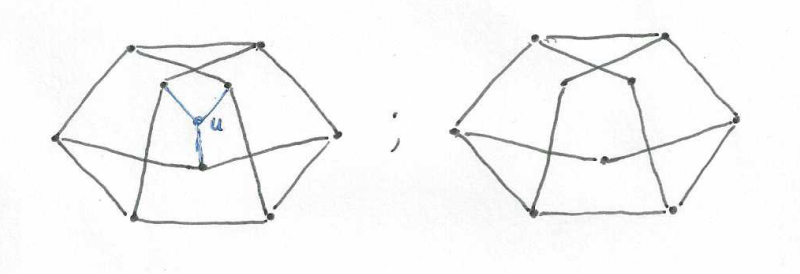
\includegraphics{Capture}
						\end{center}
						Observe that the resulting subgraph is a subdivision of $K_{3, 3}$. Thus, the Petersen graph is nonplanar by Kuratowski's Theorem.

					\item[\textbf{iii.}] Since we know that the bound in \textbf{i} is tight, it suffices to remove the lowest number of edges that satisfies the bound and also can
						be verified via an illustration. Observe that removing a single edge will not satisfy the bound as we cannot lower the girth. In fact, two edges is required.
						\begin{center}
							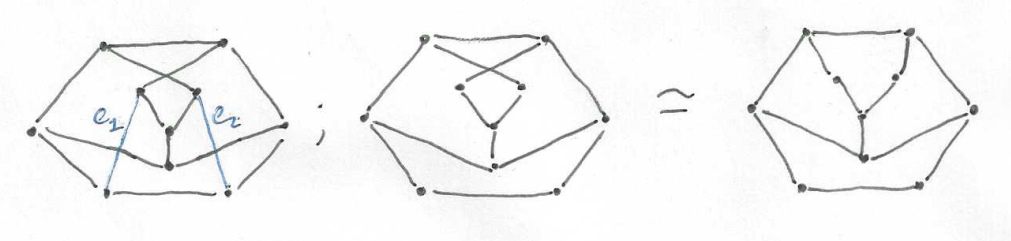
\includegraphics{Capture1}
						\end{center}
				\end{enumerate}
			\end{proof}


		% problem 5
		\item[\textbf{5.}] A graph is \textit{outerplanar} if and only if it has a planar embedding with every vertex on the boundary of the unbounded region.
			\begin{enumerate}
				\item[\textbf{i.}] Show that every simple outerplanar graph has a vertex of degree at most two.
				\item[\textbf{ii.}] Determine the maximum number of edges in a simple outerplanar $n$-vertex graph.
				\item[\textbf{iii.}] Show that $K_4$ is planar but not outerplanar.
				\item[\textbf{iv.}] Use Kuratowski's Theorem to prove that a graph $G$ is outerplanar if and only if $G$ has no subgraph that is a subdivision of $K_4$ or $K_{2, 3}$.
			\end{enumerate}

			\begin{proof}
				\begin{enumerate}
					\item[\textbf{i.}] Suppose $G$ is a simple outerplanar graph. In the case that $G$ is a tree, then $G$ must contain a leaf. Otherwise, let $G$ contain a cycle.
						Consider the dual of $G$; let $G^*$ be the dual of $G$ induced by the finite regions of $G$ (remove the vertex associated with the infinite region). I claim
						that $G^*$ is a tree. Suppose by contradiction that $G^*$ has a cycle. Then it follows that $G$ has a cycle of boarding finite regions; however, the vertices
						that define the inner most boundary of the cycle of regions contradict the fact that $G$ is outerplanar.
						\begin{center}
							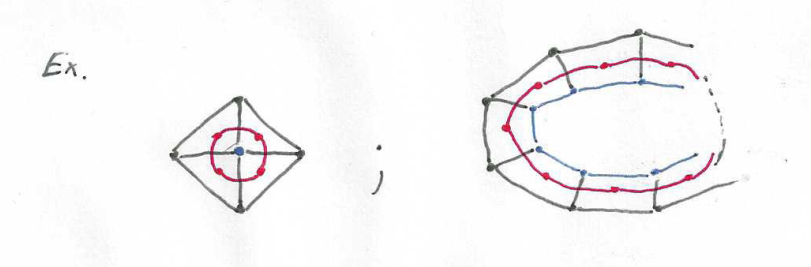
\includegraphics{Capture2}
						\end{center}
						Hence, $G^*$ is a tree as claimed. Then, we know $G^*$ must have a leaf which implies that $G^*$ has a region that boarders only one other. Since $G$ is simple,
						all regions must consist of at least three vertices. Therefore, the vertex that is not boarding the neighboring regions must have degree two.

					\item[\textbf{ii.}] I claim that the maximum number of edges in a simple outerplanar $n$-vertex graph is $2n - 3$. Let $G$ be a simple outerplanar graph with $n$
						vertices. As a base case, $n=2$, $G = P_2$ and so $e(G) = 1$ which clearly holds. For the inductive step, suppose $e(H) \leq 2(n-1) - 3$ for all simple
						outerplanar graphs $H$. Now, let $V(G) = [n]$. Observe that any subgraph of an outerplanar graph is also outerplanar; since the removal of edges and vertices
						of an outerplanar graph will not remove a vertex from the boundary of the unbounded region, it must hold that any subgraph is also outerplanar. Additionally,
						there must exist a vertex $u \in V(G)$ such that $d(u) \leq 2$. Removing $u$ from $G$ provides $H = G - x$. Thus, $$e(G) \leq e(H) - 2 \leq 2n - 2.$$

					\item[\textbf{iii.}] Observe that $K_4$ can be illustrated as [insert photo]. Therefore, $K_4$ is planar by definition. In regard to outerplanarity, suppose by
						contradiction that $K_4$ is outerplanar. Then it must hold that $e(K_4) \leq 2n - 3$ via \textbf{ii}; however, $$e(K_4) = 6 \geq 5 = 2n - 3.$$

					\item[\textbf{iv.}] [Missing proof].
				\end{enumerate}
			\end{proof}


		% problem 6
		\item[\textbf{6.}] A \textit{permutation matrix} $P$ is a binary matrix having exactly one 1 in every row and column. Prove that any square matrix of nonnegative integers can be
			expressed as the sum of $k$ permutation matrices if and only if all rows sums and column sums are equal to $k$.

			\begin{proof}
				Suppose we have a matrix $A_{n \times n}$ which can be expressed as a sum of $k$ permutation matrices. Then clearly all of its row sums and columns sums will sum to $k$
				since there is a 1 for every row and column in every particular matrix. \\ \\
				Conversely, suppose we have a matrix $A_{n \times n}$ with nonnegative terms where its row and column sums all individually sum to $k$. Consider a bipartite graph
				$G[X, Y]$ where $X = [n^2]$ for every entry in the matrix, $Y = [n^3]$ for all possible permutation matrices, and an edge $xy$ is drawn if the entry $x$ needs... \\
				Unfinished.
			\end{proof}
\end{enumerate}

\end{document}